\section*{セキュリティモジュール:電子錠}


\uline{概要}:対になっている赤と青の接続プレートでできているロックが5つあります。また5つの絞りと一つのスイッチがあります。

\begin{center}
    
\includegraphics[width=0.6\textwidth]{images/13.png}
\end{center}

\begin{textblock*}{5cm}(2.6cm,9.1cm)
    \tegakifont インシュレータ
\end{textblock*}
\begin{textblock*}{5cm}(1.4cm,11cm)
    \tegakifont 記号が書いている絞り
\end{textblock*}
\begin{textblock*}{5cm}(15.5cm,7.3cm)
    \tegakifont ロック
\end{textblock*}
\begin{textblock*}{5cm}(15.5cm,9.8cm)
    \tegakifont スイッチ
\end{textblock*}


\uline{解除方法}:正しいロックを開き{、}モジュールに電流を流します。\\
ロックごとに{、}次の手順を1つずつ実行します。\\
\begin{enumerate}
    \item (青または赤の接続プレートをドラッグして)慎重にロックを開き{、}ロックの下の絞りが開きます。
    \item 次のページのリストのいずれかで記号を見つけます。
    \item 記号がロックが開いている必要があることを示している場合(断絶記号){、}ロックの接続プレートの間にインシュレータを配置し(接続プレート間の円を押します){、}次のロックに進みます。
    \item 記号がロックを閉じている必要があることを示している場合(連結記号){、}ロックを閉じて{、}次のロックに進みます。
\end{enumerate}

最後に{、}電源スイッチを押して電源を入れます。 正しいロックが開閉されている場合{、}モジュールは解除されます。

「まだ生きている爆発物処理班」の為のヒント:
\begin{itemize}
    \item[$\bullet$] ショートしないように注意!ロックの接続プレートを広げすぎたときにショートが発生します。
    \item[$\bullet$] 記号をよく見てください。誤解を招く可能性があります…
    \item[$\bullet$] 間違えた場合は{、}もう一度押してインシュレータを取り外すことができます。
\end{itemize}

\newpage

{\large 断絶記号:ロックが開いている必要があります。インシュレータを配置してください。}
\begin{center}
    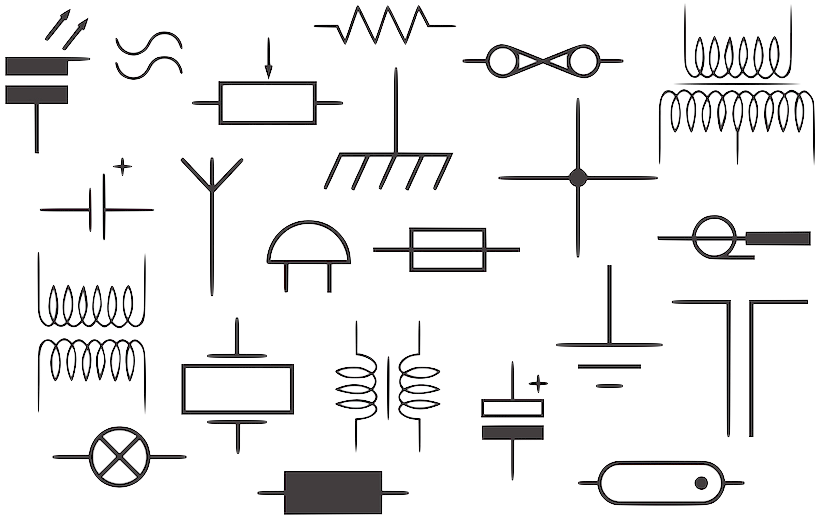
\includegraphics[width=\textwidth]{images/14.png}
\end{center}

{\large 連結記号:ロックが閉じている必要があります。}
\begin{center}
    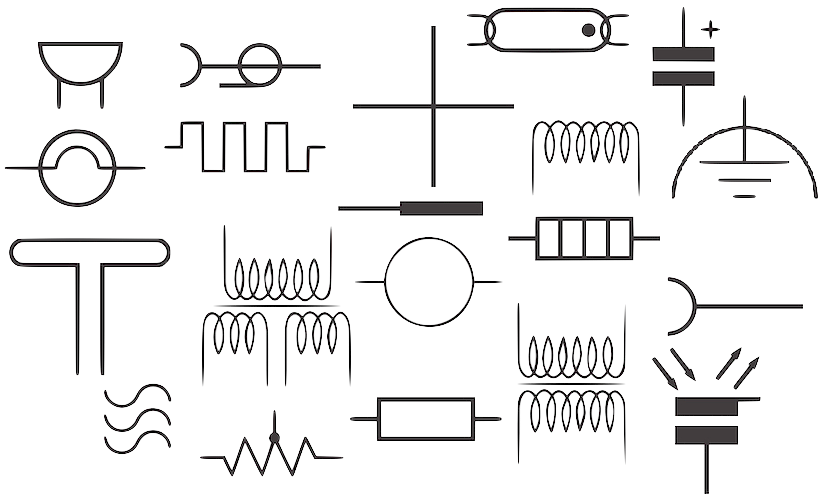
\includegraphics[width=\textwidth]{images/15.png}
\end{center}

